\documentclass{article}
\usepackage[utf8]{inputenc}
\usepackage{indentfirst}
\usepackage{enumitem, amsmath, amssymb}
\usepackage[a4paper, margin=0.8in]{geometry}
\usepackage{graphicx, caption}

\graphicspath{ {./images/} }


\title{Algebraic Topology  --- Feedback Exercise 5}
\author{Samuel Jackson --- 2520998j}
\date{\today}

\begin{document}

\maketitle

\newcommand{\R}{\mathbb{R}}
\newcommand{\Z}{\mathbb{Z}}
\newcommand{\N}{\mathbb{N}}
\newcommand{\fund}{\pi_1}
\newcommand{\pind}{p_{\ast}}


%%%
\begin{center}
    \section*{Question (1)}
\end{center}

\begin{flushleft}
	\begin{enumerate}[label=\alph*)]
		\item For the given case of $X$, a wedge sum of two circles, we have one vertex. Define $X$ as in the image below:  
		\begin{center}
			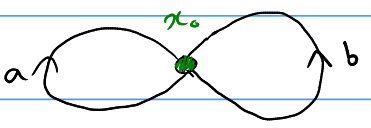
\includegraphics[height=2cm, width=6cm]{images/original-X.png}
		\end{center}
		The vertex, and basepoint, $x_0$ has an input and an output for directed edges $a$ and $b$. A five-sheeted covering requires that every point $x \in X$ has 5 elements in the preimage. The two coverings below are 5-sheeted coverings (denoted $H, K$ respectively):
		
		\begin{center}
			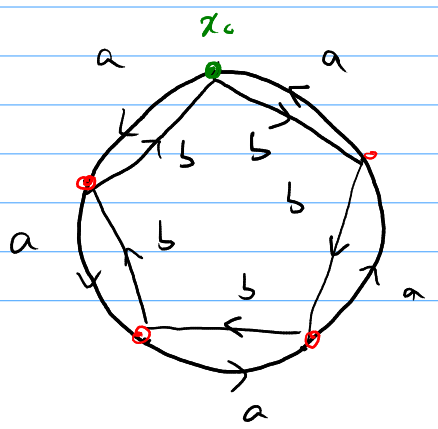
\includegraphics[height=3cm, width=3.5cm]{images/circular-sheet-covering.png}
		\end{center}
		\begin{center}
			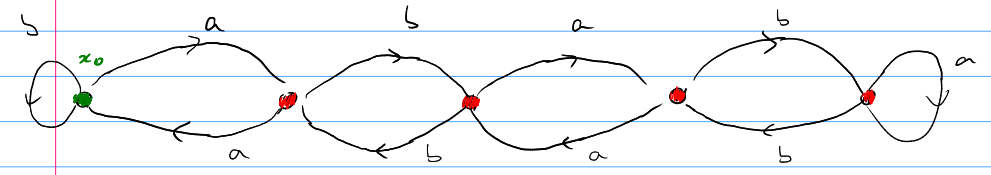
\includegraphics[height=3cm, width=13cm]{images/chain-sheet-covering.png}
		\end{center}
		(Apologies, I could not get them to look nice together).
		
		For each vertex, coloured red or green, there is an outgoing $a$ and $b$ edge alongside an ingoing $a$ and $b$ edge. Note that the edges on end vertices of the chain-based covering are both ingoing and outgoing edges.
		
		These are clearly not homeomorphic since $a^2$ (from $X$) lifts to a loop with the chain-sheet covering but does not lift to a loop in the circular-sheet covering.
		
		\item The covering $H$ permits a spanning tree which travels anti-clockwise along the $a$ edges. Using the spanning tree, we find the generators for $H$ to be $A := \{ab, a^2ba^{-1}, a^3ba^{-2}, a^4ba^{-3}, a^4b^{-1}, a^5\}$. Then, the elements of $A$ generate a subgroup of $\fund(X, x_0)$.
		
		Similarly, for the covering $K$, a spanning tree which travels along the top edges, alternating $a$ and $b$, provides the generators $B := \{b, a^2, ab^2a^{-1}, aba^2b^{-1}a^{-1}, abab^2a^{-1}b^{-1}a^{-1}, ababab^{-1}a^{-1}b^{-1}a^{-1}\}$. Hence, we have the subgroup of $\fund(X, x_0)$ generated by the elements of $B$.
	\end{enumerate}
\end{flushleft}
%%%
\begin{center}
    \section*{Question (2)}
\end{center}

\begin{flushleft}
	\begin{enumerate}[label=\alph*)]
		\item For the given $X$, $\Delta_0(X) = \langle t, u, w, v, x, y, z\rangle$, $\Delta_1(X) = \langle a, b, c, d, e, f ,g\rangle$ and finally $\Delta_2(X) = 0$, the trivial group. \newline 
		
		We define $\partial_1$ to be $\partial_1: \Delta_1(X) \rightarrow \Delta_0(X)$. For an edge $p$, $\partial_1(p) = p_1 - p_0$, where $p_0, p_1$ are the start and end of the edge respectively. \newline 
		
		Similarly, $\partial_2: \Delta_2(X) \rightarrow \Delta_1(X)$. However, since $\Delta_2$ is the trivial group, $\partial_2$ is the trivial homomorphism.
		
		This gives us the groups $\ker(\partial_1) = \langle d, e, f - g\rangle$ and $\text{im}(\partial_1) = \langle t-w, u-w, z-y, v-w\rangle$. 
		\item By definition of $H_0(X)$, we have $H_0(X) = \Delta_0(X) / \text{im}(\partial_1)$ = $\langle t, u, w, v, x, y, z : t=w, u=w, v=w, z=y\rangle$ = $\langle w, x, y \rangle \cong \Z^3$.
		\item Similar to last question, by definition $H_1(X) = \ker(\partial_1) / \text{im}(\partial_2)$. Since $\Delta_2(X)$ is the trivial group, the homomorphism is the trivial homomorphism, hence $\text{im}(\partial_2) = 0$. Then, $H_1(X) = \ker(\partial_1) = \langle d, e, f - g\rangle \cong \Z^3$.
	\end{enumerate}
\end{flushleft}
\end{document}
